\chapter{实验和数值结果}

在本章中,我将使用 Y. Pourasad 等人的实验结果所提出的算法步骤的结果,如图 1 所示。
在第一步中,导入大小为$m\times n$的输入灰度图像。
基于图\ref{fig:4.1}\footnote{(顺带当作是脚注示例)注意给图片标签命名时不要像我这样使用4.1,
不然如果你要在前面加图片会导致很混乱,最好起别的名字},使用使用的两个逻辑图创建了一个混沌序列。
最后,在扩散步骤中,生成用于加密的安全密钥。
对于输入图像的加密,必须在小波分解子带之间插入安全密钥。 
DWT方法的子带如图\ref{fig:4.1}所示。DWT子带中从上到下和从左到右的图像是Low-Low、Low-High、High-Low和High-High子带。
利用二维超混沌映射 CML,产生混沌序列并进行混淆。
在最后一步,生成混淆图像。最后,图像由使用输入图像和安全密钥的加密矩阵组成。
用数值结果评估建议的算法表明该算法是稳健的。所提出算法的数值结果如表\ref{table:4.1}\footnote{
    注意给表格标签命名时不要像我这样使用4.1,
不然如果你要在前面加表格会导致很混乱,最好起别的名字(同样顺带当作是脚注示例)}所示。\\

\begin{figure}[ht]
    \begin{center}
        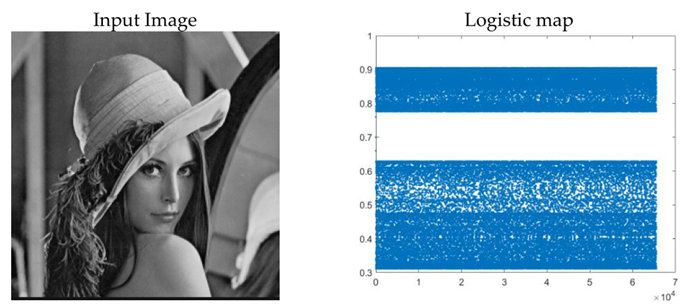
\includegraphics[width=\textwidth]{figure/p1.png}\\
        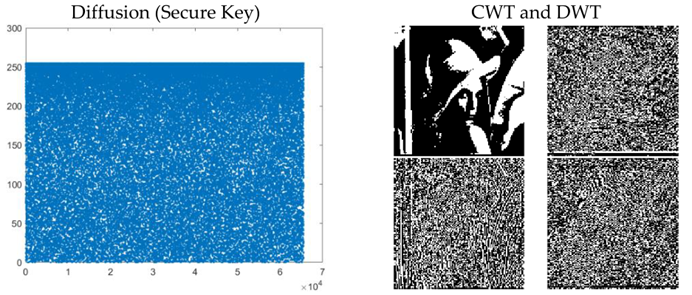
\includegraphics[width=\textwidth]{figure/p2.png}\\
        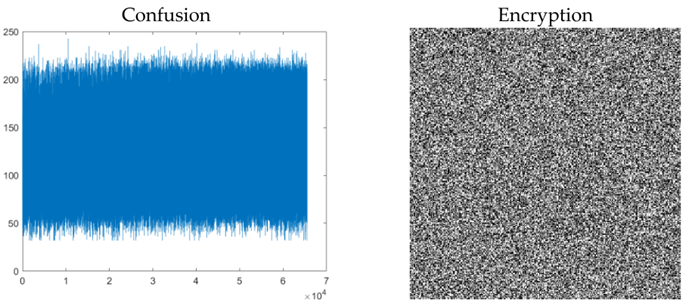
\includegraphics[width=\textwidth]{figure/p3.png}\\
    \end{center}
    \caption{所提出方法的处理结果 \label{fig:4.1}}
\end{figure}

\begin{table}[ht]
    \wuhao
    \caption{所提出的算法的数值结果 \label{table:4.1}}
    \begin{tabularx}{\textwidth}{YYYYYY}
        \Xhline{1.5pt}
        \bfseries Image & \bfseries Type & \bfseries PSNR & \bfseries NPCR & \bfseries UACI & \bfseries NC \\
        \Xhline{0.75pt}
        Lena & JPG & 42.612& 99.757 & 33.120 & 0.9548 \\
        Peppers & JPG & 39.220 & 99.787 & 33.621 & 0.9934 \\
        Barbara & JPG & 36.841 & 99.626 & 33.126 & 0.9809 \\
        Baloon & JPG & 39.134 & 99.881 & 33.415 & 0.9137 \\
        Boat & JPG & 39.223 & 99.625 & 33.671 & 0.9001 \\
        \Xhline{1.5pt}
    \end{tabularx}
\end{table}

首先,对原始图像(原始图像)进行扩散操作,主键值取自表\ref{table:4.2}。
 然后,在从表\ref{table:4.2}中获取主键值的同时执行混淆操作。 
 加密的结果与噪声相同(图\ref{fig:4.2})。 从加密图像中没有获取关于原始图像的信息。 
 通过对加密图像进行解密的密钥获取解密图像,然后进行扩散和混淆操作(图\ref{fig:4.2}(b))。\\

 \begin{table}[ht]
    \wuhao
    \caption{扩散和混淆操作的关键初始值 \label{table:4.2}}
    \begin{tabularx}{\textwidth}{YYYY}
        \Xhline{1.5pt}
        \bfseries Key (Diffusion) & \bfseries Value (Diffusion) & \bfseries Key (Confusion) & \bfseries Value (Confusion)\\
        \Xhline{0.75pt}
        $x_1(1)$ & 0.5 & $x_3(1)$ & 0.3 \\
        $x_2(1)$ & 0.5 & $y_3(1)$ & 0.3 \\
        $\mu_1$ & 4.0 & $\mu_1$ & 4.0 \\
        $\mu_2$ & 3.9 & $\mu_2$ & 3.9 \\
        \Xhline{1.5pt}
    \end{tabularx}
\end{table}

\begin{figure}[ht]
    \begin{center}
        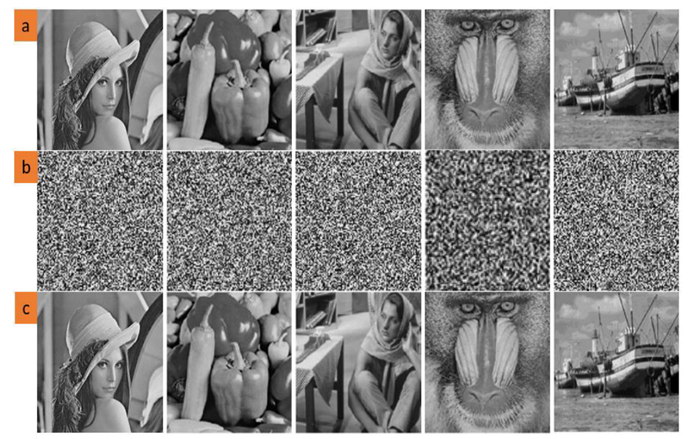
\includegraphics[width=\textwidth]{figure/p4.png}\\
    \end{center}
    \caption{将所提出的算法应用于某些图像的视觉结果\\ 
    (a) 原始图像; (b) 加密图像; (c) 重建图像 \label{fig:4.2}}
\end{figure}

\section{直方图分析}

第一个测试是加密、解密和原始图像的直方图分析。 
在这里,各个图像的图像直方图代表了加密图像和原始图像之间的巨大差异,但它们是相同的。 
通过对测试图像的直方图和加密后的直方图的评价,可以观察到加密后的图像在直方图的整个区间内是均匀分布的。 
因此,覆盖了原始图像的分布规律。 因此,有效地实施了加密(参见图\ref{fig:4.3})。

\begin{figure}[ht]
    \begin{center}
        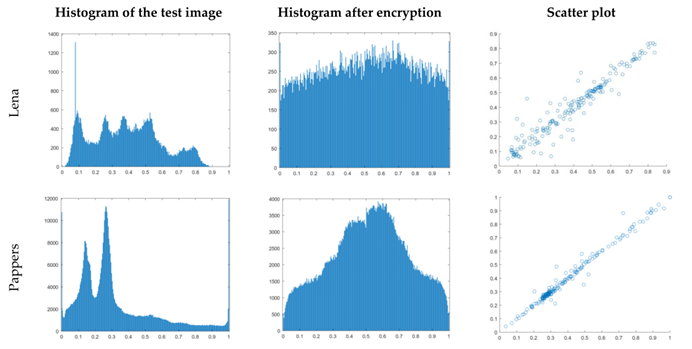
\includegraphics[width=\textwidth]{figure/p5.png}\\
        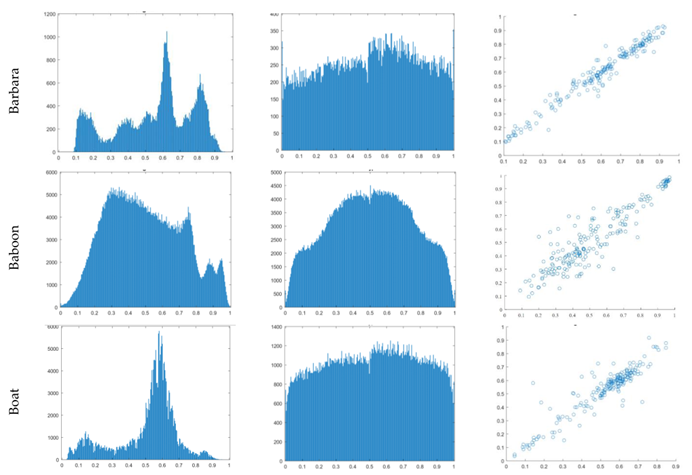
\includegraphics[width=\textwidth]{figure/p6.png}\\
    \end{center}
    \caption{原始 Lena 图像的直方图分析 \label{fig:4.3}}
\end{figure}
\section{鲁棒性 (健壮性)}

除了图\ref{fig:4.4} 中的直方图分析之外,Y. Pourasad等人还评估了输入图像和加密图像中两个垂直、
两个水平和两个对角相邻像素之间的相关性。 
图像中两个相邻像素的值由 x 轴和 y 轴表示。 
在输入图像和密码图像中,图\ref{fig:4.4}描绘了两个水平相邻像素的相关分布。 
普通图像和密码图像的相关系数分别为 0.99 和 0.02。 
对角线和垂直方向都产生相似的结果。 简单的图片具有两个相邻像素的高度相关性。

\begin{figure}[ht]
    \begin{center}
        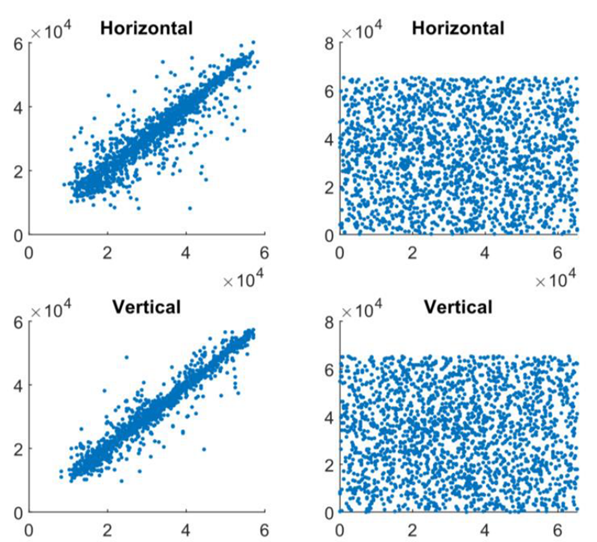
\includegraphics[width=\textwidth]{figure/p7.png}\\
        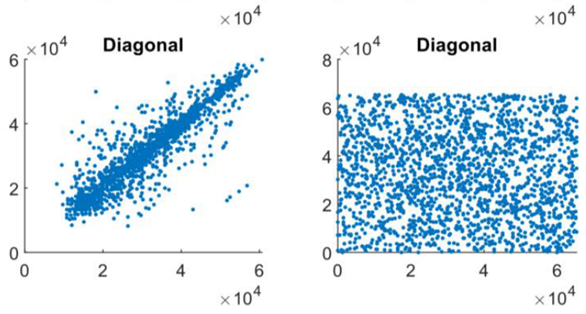
\includegraphics[width=\textwidth]{figure/p8.png}\\
    \end{center}
    \caption{Lena 图像中的像素水平、垂直和对角线、输入(左)和加密图像(右)的相关性图 \label{fig:4.4}}
\end{figure}

为了评估所提出的方法的鲁棒性,测试图像针对四种类型的图像处理攻击进行了测试:旋转、高斯噪声、中值过滤和直方图均衡。 
结果表明,所提出的设计具有更高的鲁棒性和归一化相关性。 根据结果,输入攻击不影响图像加解密。 关于不同类型图像的归
一化相关 (NC) 值,中值滤波器、旋转和高斯噪声具有更高的 NC 值。 这意味着所提出的方法的鲁棒性可以抵抗这些类型的攻
击。 然而,直方图均衡的影响是显着的(见表\ref{table:4.3})。\\

\begin{table}[ht]
    \wuhao
    \caption{所提算法在不同攻击类型下的 NC 值 \label{table:4.3}}
    \begin{tabularx}{\textwidth}{YYYYY}
        \Xhline{1.5pt}
        \bfseries Image & \bfseries Median Filter & \bfseries Histogram Equalization&\bfseries Rotation&\bfseries Gaussian Noise\\
        \Xhline{0.75pt}
        Lena & 0.984 & 0.987 & 0.999 & 0.999 \\
        Peppers & 0.704 & 0.280 & 0.923 & 0.964 \\
        Barbara & 0.914 & 0.497 & 0.980 & 0.991 \\
        Baloon & 0.960 & 0.629 & 0.991 & 0.996 \\
        Boat & 0.976 & 0.746 & 0.995 & 0.998 \\
        \Xhline{1.5pt}
    \end{tabularx}
\end{table}